\documentclass{beamer}
\mode<presentation>
  {
 %   \usetheme{Berlin}
  %\usetheme{CambridgeUS}
   \usetheme{default}
  }
  \usepackage{times}
  \usepackage{amsmath,amsthm, amssymb, latexsym}
  %\boldmath
  \usepackage[english]{babel}
  \usepackage[utf8x]{inputenc}
% use the poster package (beamerposter)
  \usepackage[orientation=portrait,size=a0,scale=1.4,debug]{beamerposter} 
  \usepackage{fancybox,pgf}
  \usepackage{tabularx}
  
\usepackage{setspace}
\usepackage{tocloft}
\usepackage{algorithm}
\usepackage{algorithmic}

\usepackage{comment}
%\usepackage[colorlinks = true,
 %           linkcolor = blue,
  %          urlcolor  = blue,
   %         citecolor = blue,
    %        anchorcolor = blue]{hyperref}
  \setbeamertemplate{navigation symbols}{}
  \setbeamertemplate{bibliography item}[text]
  \setbeamercolor*{bibliography entry author}{fg=black}
  \setbeamercolor*{bibliography item}{fg=black}
%\input compl.tex
 \RequirePackage{xspace}
 \setbeamersize{text margin left=2cm,text margin right=2cm} 
%-------------------------------------------
% 
\renewenvironment{block}[1]{%
\begin{Sbox}%
\begin{minipage}[t]{\textwidth}
~\\
\textcolor{blue}{\quad #1}~\\
~\\%
\vspace{0.5cm}
} 
{%
\end{minipage}
\end{Sbox}\Ovalbox{\TheSbox}%
}
% DEFINITIONS PRELIMINAIRES

\def\XS{\xspace}
\DeclareMathAlphabet{\mathb}{OML}{cmm}{b}{it}
\def\sbm#1{\ensuremath{\mathb{#1}}}
% Style gras italique (necessite amsmath)
%
\def\sbmm#1{\ensuremath{\boldsymbol{#1}}}
% Style gras italique (necessite amsmath)
\def\scu#1{\ensuremath{\mathcal{#1\XS}}}           % Style cursif
\def\scb#1{\ensuremath{\boldsymbol{\mathcal{#1}}}} % Style gras cursif
\usepackage{amsfonts,amssymb,amsmath,amsthm}
\usepackage{multirow}
\usepackage{graphicx}
\usepackage[footnotesize]{caption}
\usepackage{color,xspace}
\usepackage{epstopdf}
\epstopdfsetup{suffix=}
\newcommand{\dd}{
      \mathop{}\mathopen{}\mathrm{d}
   }
\newcommand{\scalegraph}{0.25}
\newcommand{\scaleimage}{0.5}   

\graphicspath{{fig/}}

%\graphicspath{{figuresFully3D2019/}}
  \title{\underline{D}ataflow \underline{A}lgorithm a\underline{R}chitecture co-design of S\underline{K}A pipeline for \underline{E}xascale \underline{R}adio \underline{A}stronomy}
  \author{ Daniel Charlet$^{**5}$ (IJCLab), Karol Desnos$^{1}$, Mickael Dardaillon$^{3}$, Andr\'e Ferrari$^{4}$, Chiara Ferrari$^{4}$, Nicolas Gac$^{3}$, Jean-Fran\c cois Nezan$^{1}$, Fran\c cois Orieux$^{3}$, Simon Prunet$^{4}$, Martin Quinson$^{2}$, Fr\'ed\'eric Suter$^{**2}$(IN2P3 Computing Center), Cyril Tasse$^{**5}$ (GEPI), C\'edric Viou$^{5}$}
  \institute{\textit{$^{1}$IETR (INSA),  $^{2}$IRISA (ENS), $^{3}$L2S (CS), $^{4}$Lagrange (UCA),  $^{5}$Nan\c cay (Obs Paris)  \\ contact: nicolas.gac@l2s.centralesupelec.fr}      }
  \date{\normalsize ISC Project Poster Session, June 30 2021}

\begin{document}

  \frame[plain]
  {
\begin{table}[t]
   \centering
\begin{tabularx}{0.99\textwidth}{cc}
  
\includegraphics[scale=0.9]{partenaires_DARK-ERA.eps} & \hspace{5cm}
   \scalebox{0.75}{ \input{fig/logo_ANR_avec_numero_projet.pdf_t}}\\   
%&
\includegraphics[scale=0.6]{logo_ANR_avec_numero_projet.pdf} \\
  \end{tabularx}
  \end{table}

\hrule
\vspace{1cm}

\begin{columns}[!]
\begin{column}{.19\linewidth}
%\vspace{1cm}

\includegraphics[scale=1.4]{DARKERA_logo_color_L.png}
\end{column}
% Second column
\begin{column}{.8\linewidth}
  \begin{minipage}{\textwidth}
	{
	\begin{center}
	\Large{\textbf{\inserttitle}}\\[1ex]
	\normalsize{\insertauthor}\\[1ex]
	\normalsize \insertinstitute\\[1ex]
	\large{\insertdate}
	\end{center}
	}
   \end{minipage}
\end{column}
\end{columns}

\vspace{1cm}
\begin{columns}[t]
\begin{column}{.49\linewidth}
\begin{block}{\large \textbf{SKA computing, an HPC challenge}}
	%\vspace{1cm}
        \begin{minipage}{0.95\textwidth}
The \textbf{exascale radio telescope} Square Kilometre Array (SKA) \cite{skatelescope} will require supercomputers with high technical demands. The Science Data Processor (SDP) pipeline in charge of producing the multidimensional images of the sky will have to execute in \textbf{realtime} a \textbf{complex algorithm chain} with data coming from telescopes at an incredible \textbf{rate of several Tb/s} and \textbf{limited storage possibilities}. The SDP will also have to be \textbf{as green as possible} with an energy budget of only 1 MWatt for 250 Petaflops. 

\begin{center}
    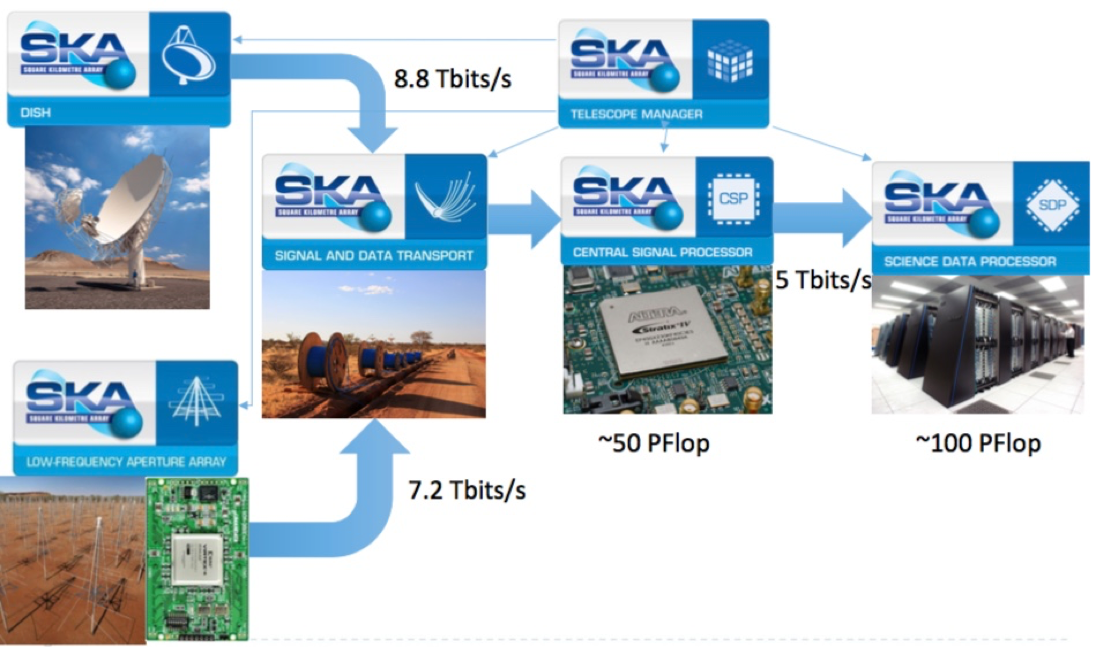
\includegraphics[width=0.9\textwidth ]{pipeline} % %et/ou [height=]
    \end{center}

The \textbf{SDP supercomputer} will be based on a standard HPC system combined with FPGA or application-specific architectures like GPU or the manycore Kalray Massively Parallel Processor Array (MPPA). One crucial challenge is to assess the performance both in time and energy of new complex scientific \textbf{dataflow algorithms} on not-yet-existing complex computing infrastructures. It will be hardly possible without efficient \textbf{co-design methods} and \textbf{rapid prototyping tools}.
\end{minipage}
\end{block}

\begin{block}{\large \textbf{Dark-Era, a 4-year project starting in 2021}}
 \begin{minipage}{0.95\textwidth}
The \textbf{consortium} gathers complementary skills in computer science, signal processing, and astronomy with twelve permanent members from the \textbf{SimGrid} \cite{casanova:hal-01017319} development Team at IRISA, the \textbf{PREESM} \cite{preesm} development team at IETR, the \textbf{inverse problem} team at L2S, and two \textbf{radio astronomy} teams at Observatories of Paris and Côte d’Azur. Dark-Era has the support of SKA-France and works in collaboration with Atos-Bull.\\

The \textbf{PhD and PostDoc positions} within Dark-Era will be published on \href{https://dark-era.pages.centralesupelec.fr}{\textcolor{blue}{https://dark-era.pages.centralesupelec.fr}} :
\begin{itemize}
    \item One post-doc at LS2 on HLS FPGA prototype (autumn 2021)
    \item Two PhDs at IETR and IRISA respectively on PREESM and SimGrid
    extensions (autumn 2022)
    \item one post-doc at Lagrange on algorithm/architecture exploration for radioastronomy (spring 2024)
\end{itemize}
 \end{minipage}
\end{block}

\begin{block}{\large \textbf{Dark-Era goals}}
 \begin{minipage}{0.95\textwidth}
 \begin{itemize}
 \item[1] Building \textbf{SimSDP}, a rapid prototyping tool providing exascale simulations from dataflow algorithm descriptions.
 \item[2] Exploring \textbf{low power accelerators} like FPGA or Kalray MPPA as alternatives to mainstream GPU architecture.
 \item[3] Being source of proposals for SKA computing and promoting French contributions such as \textbf{ddfacet} \cite{Tasse18}.
 \end{itemize}
 \end{minipage}
\end{block}

\footnotesize{
         \begin{minipage}{.99\textwidth}
        \bibliographystyle{IEEEtran}
   %      \renewcommand{\bibsection}{}
         \bibliography{bib/bib-dark-era,bib/SimGrid,bib/referencesCyril}   % bibliography data in report.bib
        % \begin{thebibliography}{50}
	%
%	\end{thebibliography}
  	\end{minipage}
  	}
\end{column}
% Second column
\begin{column}{.49\linewidth}

\begin{block}{\large \textbf{SimSDP, an exascale simulation tool}}
 \begin{minipage}{0.95\textwidth}
 \textbf{SimSDP} purpose is to provide \textbf{early analyses} in terms of memory usage, latency, throughput, and energy consumption through an original mixed approach based on execution and simulation. Following an Algorithm Architecture Matching (AAM) approach, SimSDP will rely on a dataflow model of the algorithm and a model of the target architecture. SimSDP will be based on two existing tools: PREESM and SimGrid. PREESM accurately evaluates \textbf{heterogeneous single node} performance; SimGrid accurately simulates \textbf{inter-node communications}. Their association will allow for reliable simulations of \textbf{large scale heterogeneous HPC systems}.
 \\
 \begin{center}
    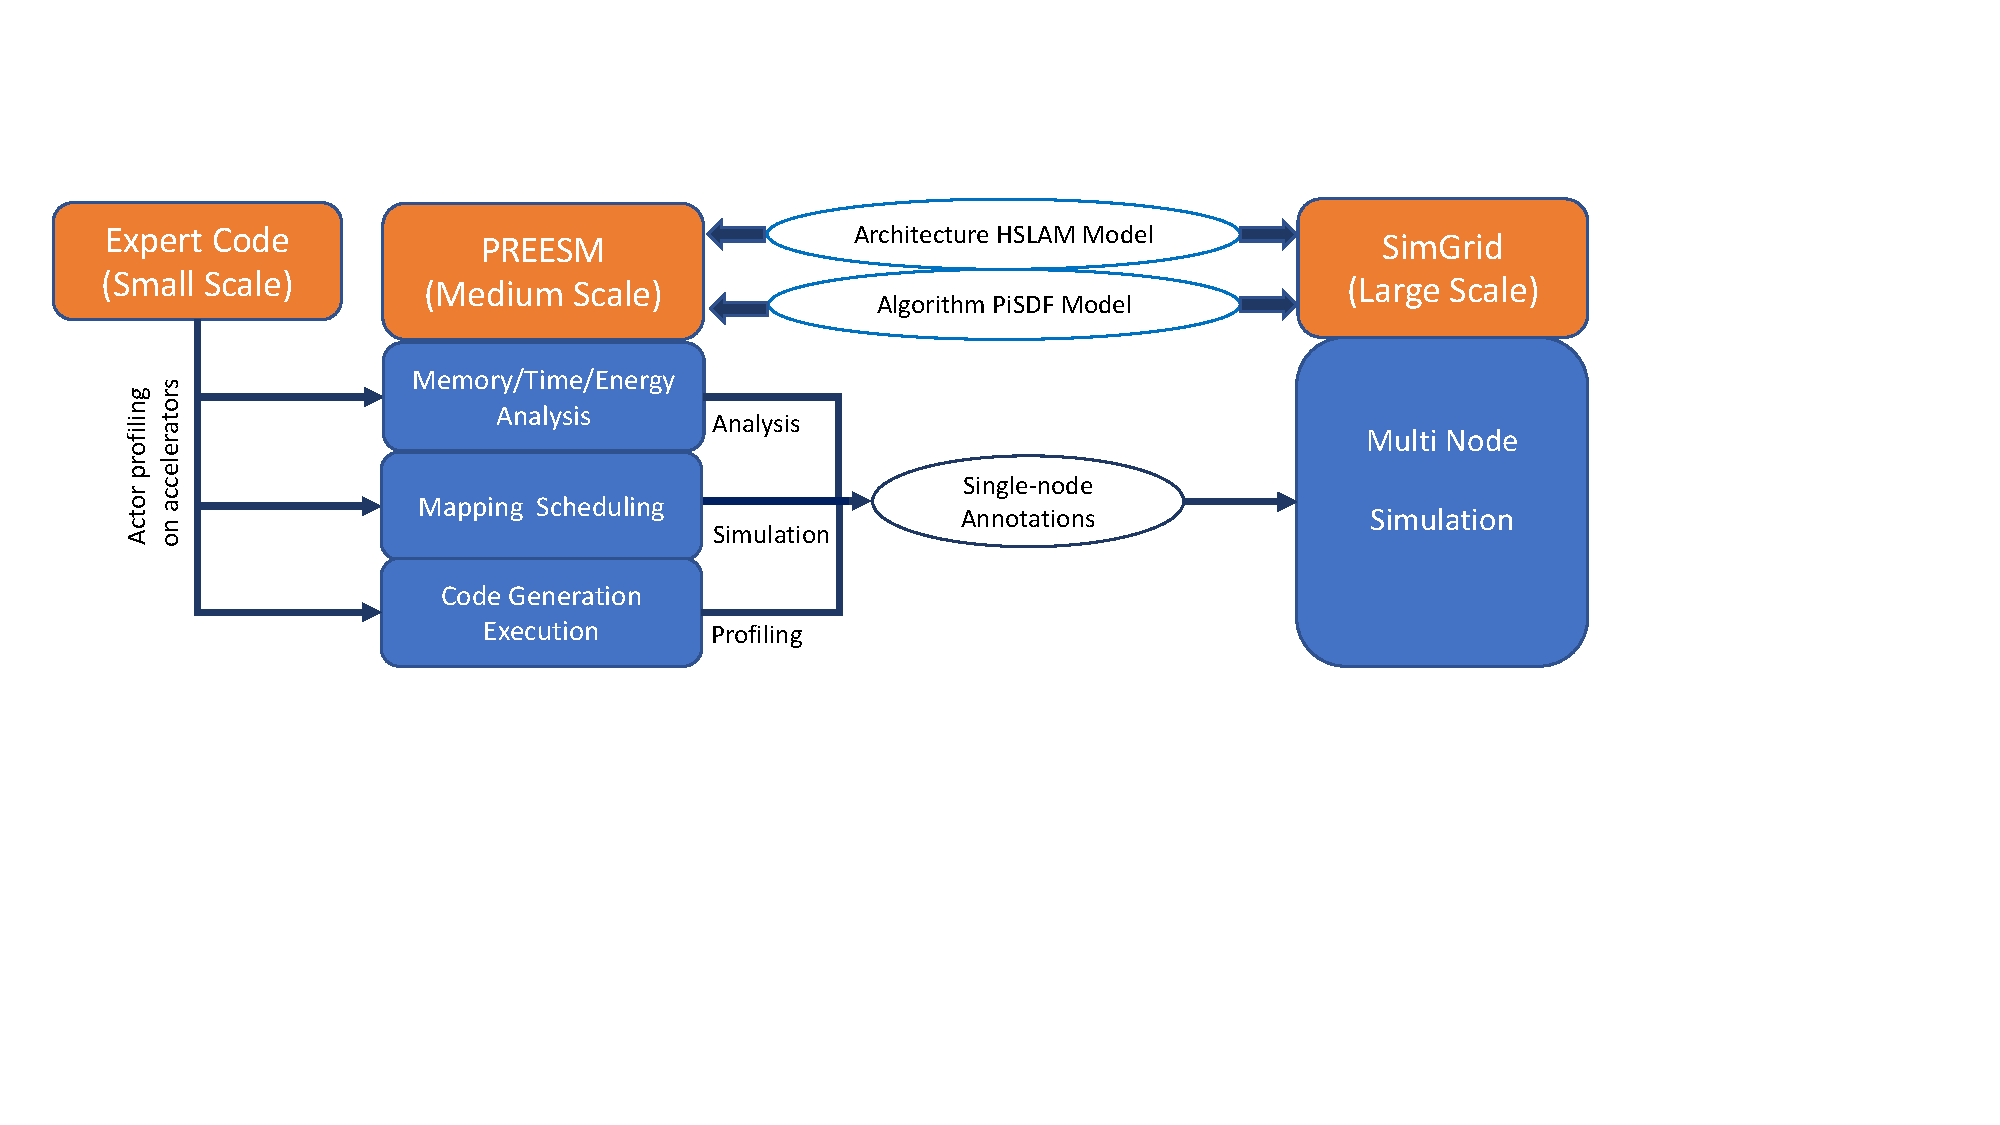
\includegraphics[width=\textwidth ]{SimSDP_overview} % %et/ou [height=]
    \end{center}
 \end{minipage}
\end{block}

\begin{block}{\large \textbf{Dark-Era tasks}}
	%\vspace{1cm}
        \begin{minipage}{0.95\textwidth}
 \begin{center}
    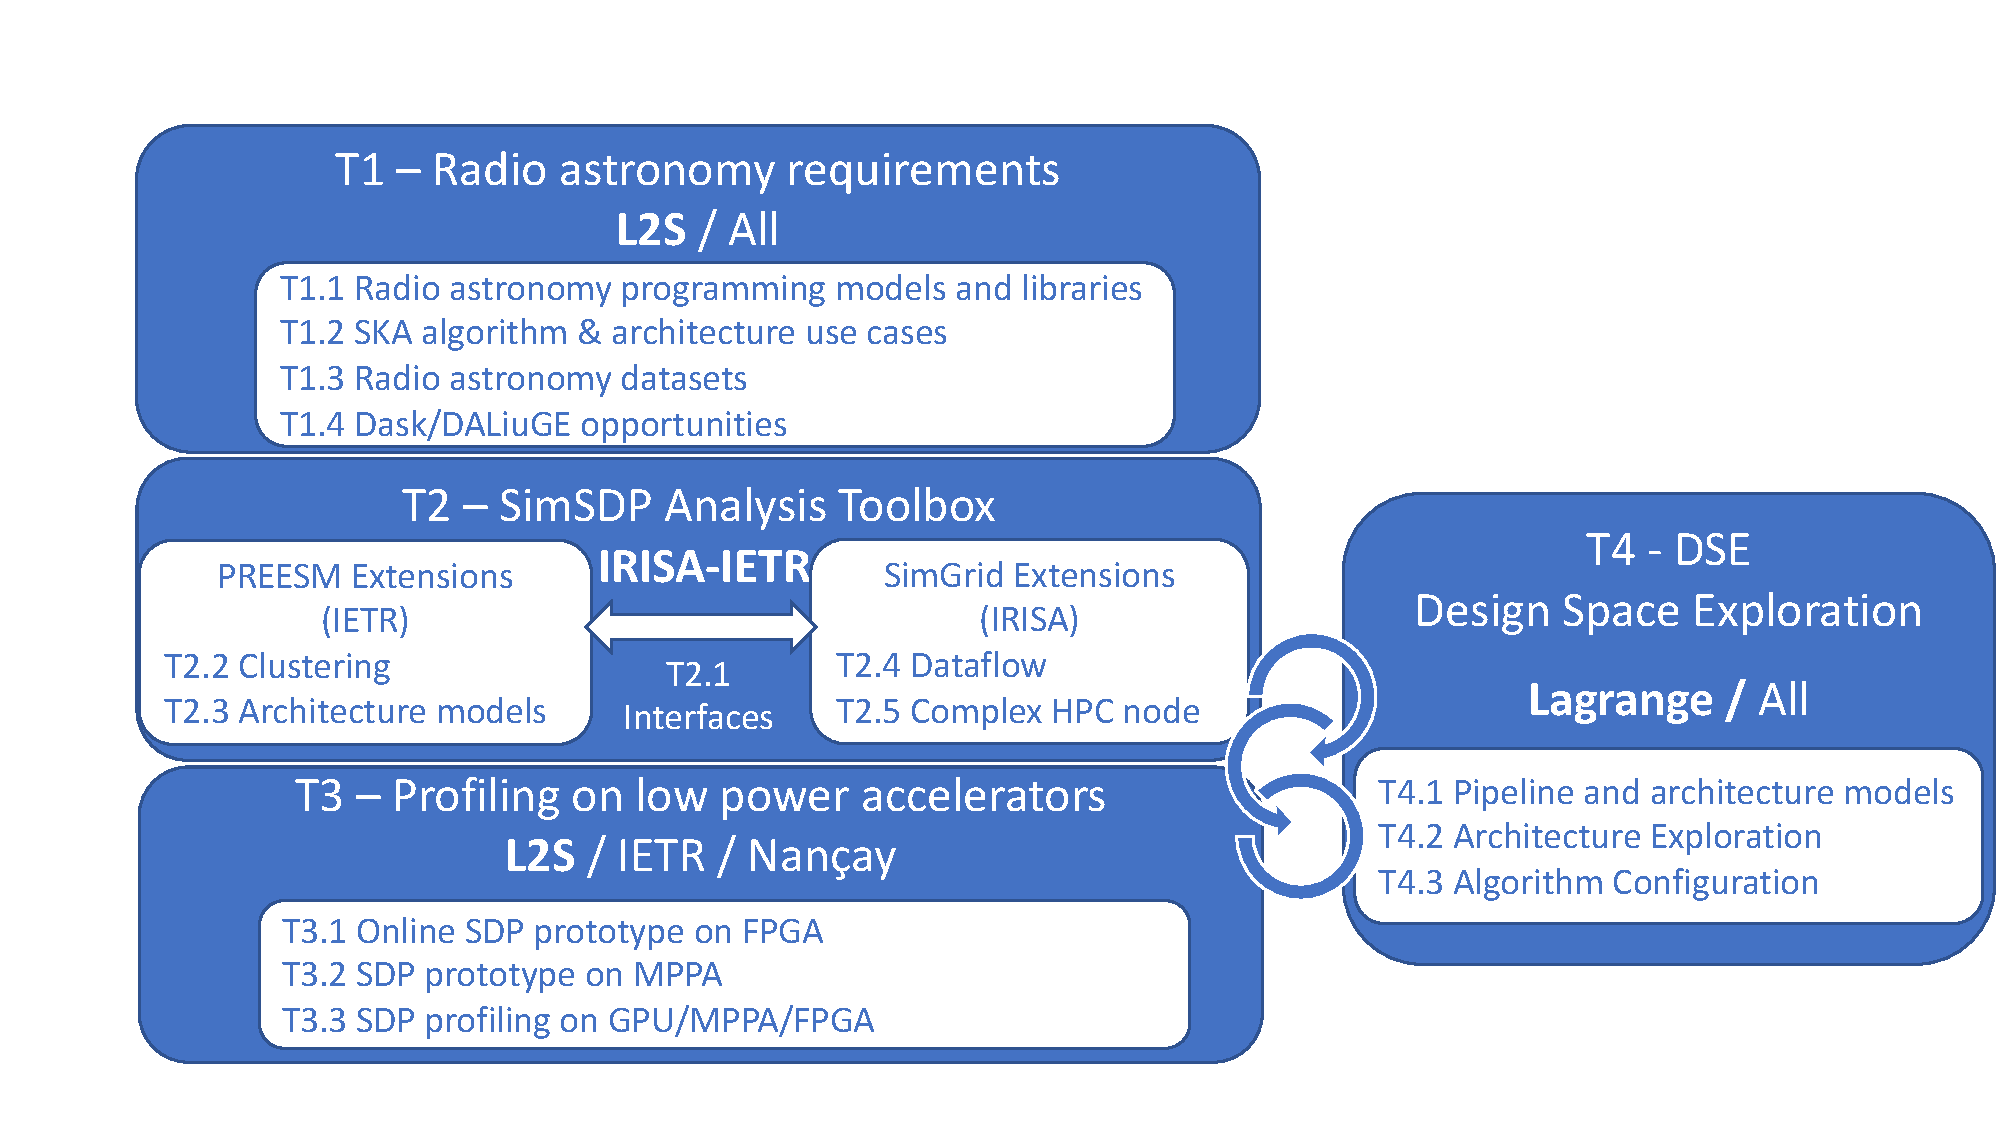
\includegraphics[width=\textwidth ]{Tasks} % %et/ou [height=]
    \end{center}
    
  
    \textbf{T1} will provide reference datasets and an SDP computing state of the art in terms of programming models, architectures and algorithms.\\
    \\
    \textbf{T2} is the core development task of the SimSDP rapid prototyping tool. New clustering and architecture model extensions in PREESM, and dataflow and complex HPC node extensions in SimGrid will be developed to improve the performance of both tools, enable seamless communication between them and, finally improve the quality of the large scale simulations.\\
    \\
In \textbf{T3}, SDP prototypes on MPPA and FPGA designed through High Level Synthesis (HLS) tools and will be developed and profiled on small scale datasets set up at the NenuFAR radio telescope. It will allow evaluating the potential of these low power accelerators. The SDP profiling feedbacks on GPU, MPPA and FPGA obtained will provide SimSDP with annotations on the dataflow graph. \\%SDP prototypes will also be compared with SimSDP simulations on medium scale datasets to evaluate SimSDP new features.\\
\\
In \textbf{T4}, algorithm and architecture spaces will be explored in the SKA context through the large scale simulations offered by SimSDP. The radio astronomy imaging pipelines will be described at a high-level of abstraction suitable for targeting any heterogeneous multinode HPC system SKA may choose in the future. Several SDP architecture configurations (number of nodes, type of accelerators) and several SDP algorithm configurations will be then explored. 
\end{minipage}
\end{block}
%\bibliographystyle{spiejour}   % makes bibtex use spiejour.bst
%\begin{block}{\large \textbf{Reference}}
%\end{block}
\end{column}
\end{columns}
}

\end{document}
